%instiki:category: FisicaSubatomica
% use latex2itexv2 chapter1.tex to obtain inkstiki file
% use latex2itexTOC to obtain Tabla de Contenidos
\chapter{Teor\'\i a Cl\'asica de Campos}
\label{chap:tcc} %noinstiki
%instiki:
%instiki:***
%instiki:
%instiki:[[NotasFS|Tabla de Contenidos]]
%instiki:
%instiki:***
%instiki:
%generated with html2itexTOC instiki_source.html
%instiki:* [Principio de M\'\i nima Acci\'on](#la)
%instiki:
%instiki:* [La cuerda cl\'asica unidimensional](#la-cuerda-clasica)
%instiki:
%instiki:* [Principio de M\'\i nima Acci\'on para ...](#principio-de-minima-call)
%instiki:
%instiki:* [Aplicaci\'on a Mec\'anica Cu\'antica](#aplic-mecan-cuant)
%instiki:
%instiki:* [Aplicaci\'on a la cuerda unidimenisonal](#aplicacion-la-cuerda)
%instiki:
%instiki:***
%instiki:
\section{Principio de M\'\i nima Acci\'on}
\label{sec:la}

El Principio de M\'\i nima acci\'on establece, una vez fijado el espacio de
coordenadas generalizadas sobre el espacio de configuraci\'on, que de
todas las trayectorias posibles que transcurren entre $t_1$ y $t_2$,
el sistema escoger\'a aquella que minimice la acci\'on $S$
\cite{ActionPhysics}.  La magnitud de la acci\'on viene dada para cada
trayectoria por la integral:
\begin{equation}
  \label{eq:la}
   S\left[q_i,\dot{q}_i\right] = \int_{t_{1}}^{t_{2}} L(q_i(t), \dot{q}_i(t),t) dt
\end{equation}
Donde:
$q_i(t)$ son las coordenadas param\'etricas de una trayectoria posible.
$L(q_i,\dot{q}_i,t)$, es la funci\'on lagrangiana del sistema.


Puede probarse mediante principios variacionales, que de todas las trayectorias posibles, la que hace  estacionaria la anterior expresi\'on es la que satisface la siguiente condici\'on $i$:
\begin{equation}
  \label{eq:eel}
 \frac{d}{dt} \left ( \frac{\partial L}{\partial\dot{q}_i} \right ) - \frac{\partial L}{\partial q_i} = 0
\end{equation}
conocidas como las ecuaciones de Euler-Lagrange. La demostraci\'on se
har\'a m\'as adelante para el caso en el que las coordenadas generalizadas
corresponden a funciones de campo. 

De momento mostraremos como la segunda ley de Newton~\cite{NewtonSeconLaw}, puede escribirse en la forma de la ec.~(\ref{eq:eel}).
\begin{align}
\label{eq:fma}
  F&=ma\\
  -\frac{\partial V(x)}{\partial x}&=m\frac{d^2x}{dt^2}\nonumber\\
  &=m\frac{d\dot{x}}{dt}\nonumber\\
  &=\frac{d}{dt}
  \left[
    \frac{\partial}{\partial\dot{x}}
    \left(
      \frac{1}{2}m\dot{x}^2
    \right)
  \right]\nonumber
\end{align}
Podemos introducir el Lagrangiano a cada lado de la igualdad adicionando t\'erminos con la respectiva derivada parcial cero:
\begin{equation*}
  \frac{\partial}{\partial x}
  \left(
\frac{1}{2}m\dot{x}^2-V(x)
  \right)=\frac{d}{dt}
  \left[
    \frac{\partial}{\partial\dot{x}}
    \left(
      \frac{1}{2}m\dot{x}^2-V(x)
    \right)
  \right].
\end{equation*}
Reemplazando $L=\frac{1}{2}m\dot{x}^2-V(x)=T-V$, obtenemos
\begin{equation*}
\frac{d}{dt}\frac{\partial L}{\partial\dot{x}}  -\frac{\partial L}{\partial x}=0.
\end{equation*}
Una forma m\'as rigurosa de escribir la ec.~\eqref{eq:fma} puede encontrarse en~\cite{ActionPhysics}. 

El Hamiltoniano del sistema se obtiene definiendo la variable can\'onica conjugada de $x$
\begin{align}
  p=\frac{\partial\mathcal{L}}{\partial\dot{x}}=m \dot{x},
\end{align}
y usando la transformada de Legendre
\begin{align}
  H=p \dot{x}-L=\frac{\partial\mathcal{L}}{\partial\dot{x}}\dot{x}-L=\frac{1}{2}m\dot{x}^2+V=T+V
\end{align}

Para visualizar el principio de m\'\i nimo de acci\'on se recomienda seguir las actividades del programa interactivo en \texttt{Java} disponible online en \cite{JavaAP}. All\'\i{} se considera el problema de un objeto de 0.2Kg lanzado hacia arriba y retornado al punto de partida 3 segundos despues. Si dividimos la trayectoria en tres intervalos como se muestra en la Fig.~\ref{fig:apple1}, teniendo en cuenta que la velocidad es la pendiente del segmento, para $\Delta t=0.75\,$s $x_1=11.13\,$m, $t_1=0.75\,$s, $x_2=0\,$m, $t_2=1.5\,$s, tenemos que para la trayectoria mostrada
\begin{align}
  S=\int_{t_1}^{t_2}(T-V)dt\approx&\sum_i(T-V)_i\Delta t\nonumber\\
  \approx&\sum_{i=1}^2\left[\frac{1}{2}m\left(\frac{x_i-x_{i-1}}{t_i-t_{i-1}}\right)^2-m g x_i\right]\Delta t\nonumber\\
  \approx&16.67\,\text{J\,s}
\end{align}
\begin{figure}
  \centering
  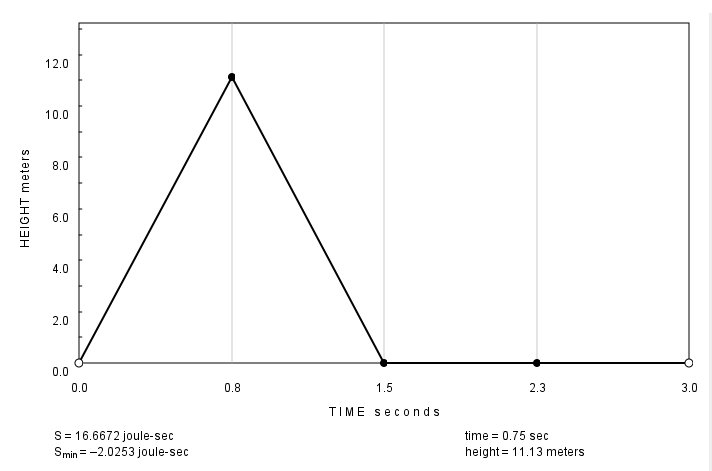
\includegraphics[scale=0.5]{apple1}
  \caption{Ejemplo de c\'alculo de la Acci\'on para una trayectoria arbitraria}
  \label{fig:apple1}
\end{figure}
Iterando el proceso se puede encontrar num\'ericamente (o a mano) la trayectoria que minimiza la acci\'on mostrada en la Fig.~\ref{fig:apple2}
\begin{figure}
  \centering
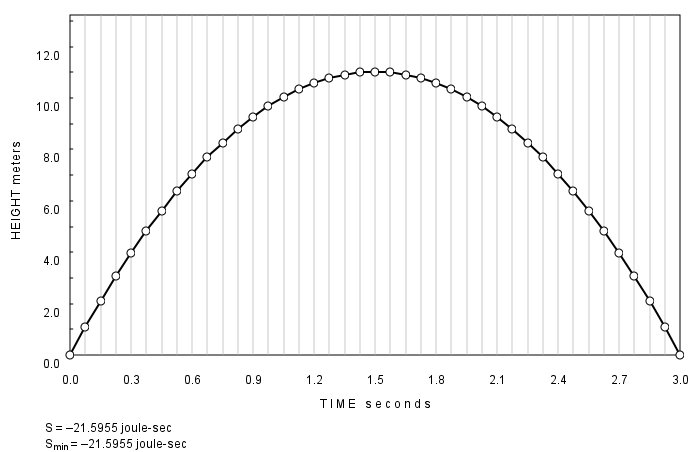
\includegraphics[scale=0.5]{apple2}
  \caption{Trayectoria que minimiza la Acci\'on}
\label{fig:apple2}
\end{figure}
Para una dimensi\'on podemos definir la densidad Lagrangiana como
\begin{equation}
  \mathcal{L}(q,\dot q,t)=\frac{\partial}{\partial q}L(q,\dot q,t)\qquad\text{or}\qquad L(q,\dot q,t)=\int\mathcal{L}(q,\dot q,t)dq.
\end{equation}
La ec.~\eqref{eq:la} puede escribirse entonces como
\begin{equation}
   S\left[q_i,\dot{q}_i\right] = \int \mathcal{L}(q_i(t), \dot{q}_i(t),t)\, dq\,dt.
\end{equation}
Para sistemas continuos es conveniente usar la densidad Lagrangiana. Abordaremos a continuaci\'on el sistema continuo correspondiente a la cuerda cl\'asica unidimensional para construir la densidad Lagrangiana correspondiente. A partir de ella demostraremos las ecuaciones de Euler Lagrange para dicho sistema.

%\left(\right)

\section{La cuerda cl\'asica unidimensional}
\label{sec:la-cuerda-clasica}

Considere una cuerda de longitud $L$ formando un c\'\i rculo de radio $R$.
Es conveniente considerar un conjunto de $N$ part\'\i culas de masa $m$ a
lo largo de la circunferencia, unidas por resortes de longitud $l$ y
constante el\'astica $k$. Los modos vibracionales de la cuerda a lo
largo de la circunferencia se obtienen en l\'\i mite de $N\to\infty$ y $l\to0$ 
%noinstiki

\begin{figure} %noinstiki
  \centering %noinstiki
  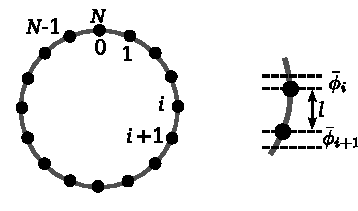
\includegraphics{cuerda} %noinstiki
  \caption{Modelo Cuerda} %noinstiki
  \label{fig:1string} %noinstiki
\end{figure} %noinstiki<div id="fig:1string">Figura cuerda: Modelo cuerda</div>
%noinstiki![cuerda](http://gfif.udea.edu.co/figfs/cuerda.png)
%noinstiki
De acuerdo a la figura 
\ref{fig:1string}, %noinstiki([cuerda](#fig:1string)),
si $\bar{\phi_i}=\bar{\phi}(z_i,t)$ es el
desplazamiento de la $i$--esima masa desde su posici\'on de equilibrio,
entonces el Lagrangiano del sistema de $N$ particulas y resortes es:
\begin{align}
  \label{eq:1strLsum} %noinstiki
  L&=\frac{1}{2}m\sum_{i=0}^{N-1}
  \left(
\frac{\partial\bar\phi_i}{\partial t}
  \right)^2-\frac{1}{2}k\sum_{i=0}^{N-1}
  \left(
\bar\phi_{i+1}-\bar\phi_{i}
  \right)^2,\\
  \label{eq:1strLsumdot} 
&=\frac{1}{2}m\sum_{i=0}^{N-1}
  \left(
    \dot{\bar{\phi_i}}
  \right)^2-\frac{1}{2}k\sum_{i=0}^{N-1}
  \left(
\bar\phi_{i+1}-\bar\phi_{i}
  \right)^2.
\end{align}
Si $\mu$ es la densidad de la cuerda, $T$ la tensi\'on y $v$ la velocidad, entonces
\begin{align}
  \label{eq:micromacro}
  \mu&=\frac{m}{l}\nonumber\\
  T&=kl\\
  v^2&=\frac{T}{\mu}.\nonumber
\end{align}
(\ref{eq:micromacro})
En el l\'\i mite $l\to0$ y $N\to\infty$, tenemos
\begin{equation}
  \label{eq:barf}
  \bar\phi_i=\bar\phi(z_i,t)\to\bar\phi(z,t),
\end{equation}
que representa la funci\'on de campo del desplazamiento de una masa
infinitesimal de su posici\'on de equilibrio. Entonces
\begin{align}
L&=\frac{1}{2}\sum_{i=0}^{N-1}\frac{m}{l}l
  \left(
    \dot{\bar{\phi_i}}
  \right)^2-\frac{1}{2}\sum_{i=0}^{N-1}(k l) l
  \left(
\frac{\bar\phi_{i+1}-\bar\phi_{i}}{l}
  \right)^2.\nonumber\\
&=\frac{1}{2}\sum_{i=0}^{N-1}\mu
  \left(
    \dot{\bar{\phi_i}}
  \right)^2l-\frac{1}{2}\sum_{i=0}^{N-1}T
  \left(
\frac{\bar\phi_{i+1}-\bar\phi_{i}}{l}
  \right)^2l.
\label{eq:1strLsumm}
\end{align}
En el l\'\i mite continuo $\sum(\cdots)\,l\to\int(\cdots)\,dz$, entonces 
\begin{equation}
\label{eq:238}
  L=\int_0^L\frac{1}{2}
\left[
  \mu\left(\frac{\partial\bar\phi}{\partial t}\right)^2- T\left(\frac{\partial\bar\phi}{\partial z}\right)^2
\right]dz=\int_0^L\mathcal{L}dz,
\end{equation}
con
\begin{equation}
  \label{eq:call1}
  \mathcal{L}=\frac{1}{2}
\left[
  \mu\left(\frac{\partial\bar\phi}{\partial t}\right)^2- T\left(\frac{\partial\bar\phi}{\partial z}\right)^2
\right],
\end{equation}
y
\begin{equation}
  \label{eq:Scall}
  S=\int\mathcal{L}\,dtdz.
\end{equation}
Definiendo
\begin{equation}
  \label{eq:barff}
  \phi=\sqrt{T}\bar\phi,
\end{equation}
tenemos
\begin{align}
  \label{eq:call2}
  \mathcal{L}(\partial\phi/\partial t,\partial\phi/\partial z)=&
\frac{1}{2}
\left[
  \frac{\mu}{T}\left(\frac{\partial\phi}{\partial t}\right)^2- \frac{T}{T}\left(\frac{\partial\phi}{\partial z}\right)^2
\right]\nonumber\\
=&\frac{1}{2}
\left[
  \frac{1}{v^2}\left(\frac{\partial\phi}{\partial t}\right)^2-\left(\frac{\partial\phi}{\partial z}\right)^2
\right],
\end{align}
Note que:
\begin{align}
  \label{eq:dcalt}
  \frac{\partial}{\partial t}
  \left[
    \frac{\partial\mathcal{L}}{\partial
      (\partial\phi/\partial t)}
  \right]&=    \frac{1}{v^2}\frac{\partial^2\phi}{\partial t^2}\\
  \label{eq:dcalz} %noinstiki
  \frac{\partial}{\partial z}
  \left[
    \frac{\partial\mathcal{L}}{\partial
      (\partial\phi/\partial z)}
  \right]&= -\frac{\partial^2\phi}{\partial z^2}
\end{align}


Si en la ec.~\eqref{eq:1strLsumdot}, tomamos como coordenadas
generalizadas las $N$ $\dot{\bar{\phi_i}}$ y $\bar\phi_i$, entonces, podemos
obtener las ecuaciones de movimiento a partir de las ecuaciones de
Euler-Lagrange \eqref{eq:eel}:
\begin{equation}
  \label{eq:eelfi}
   \frac{d}{dt} \left ( \frac{\partial L}{\partial\dot{\bar{\phi_i}}} \right ) -
   \frac{\partial L}{\partial \bar\phi_i} = 0,
\qquad \text{$i=0$ hasta $N-1$}.
\end{equation}
En el l\'\i mite $l\to0$ y $N\to\infty$, y usando las ecs.~\eqref{eq:dcalt} 
y \eqref{eq:dcalz}, %noinstiki
\begin{align}
  \label{eq:emov1}
  \frac{d}{dt} \left( \frac{\partial L}{\partial\dot{\bar{\phi_i}}} \right)
  &=\frac{d}{dt} \left( m\dot{\bar{\phi_i}} \right)
= m\frac{\partial^2\bar{\phi_i}}{\partial t^2} \nonumber\\
&= T l\left(\frac{\mu}{T}\frac{\partial^2\bar{\phi_i}}{\partial t^2} \right)\nonumber\\
  &\to
  l\sqrt{T}
  \left(
    \frac{1}{v^2}\frac{\partial^2\phi}{\partial t^2}
  \right)\\
  \label{eq:eecalt} %noinstiki
  &=l\sqrt{T}\frac{\partial}{\partial t}
  \left[
    \frac{\partial\mathcal{L}}{\partial
      (\partial\phi/\partial t)}
  \right].
\end{align}
Para el segundo t\'ermino de la ec.~(\ref{eq:eelfi}) n\'otese que
\begin{align}
- \sum_{i=0}^{N-1}\left(\bar\phi_{i+1}-\bar\phi_{i}\right)^2= 
 &-\left(\bar\phi_{1}-\bar\phi_{0}\right)^2-\left(\bar\phi_{2}-\bar\phi_{1}\right)^2-\cdots
-\left(\bar\phi_{(i-1)+1}-\bar\phi_{i-1}\right)^2-\left(\bar\phi_{i+1}-\bar\phi_{i}\right)^2-\cdots\nonumber\\
 =&-\left(\bar\phi_{1}-\bar\phi_{0}\right)^2-\left(\bar\phi_{2}-\bar\phi_{1}\right)^2-\cdots
 -\left(\bar\phi_{i}-\bar\phi_{i-1}\right)^2-\left(\bar\phi_{i+1}-\bar\phi_{i}\right)^2-\cdots\nonumber\\
\end{align}
Entonces
\begin{align}
-\frac{\partial}{\partial\bar\phi_i}  \sum_{i=0}^{N-1}\left(\bar\phi_{i+1}-\bar\phi_{i}\right)^2
=&-2\left(\bar\phi_{i}-\bar\phi_{i-1}\right)-2\left(\bar\phi_{i+1}-\bar\phi_{i}\right)\times(-1)\nonumber\\
=&2l\left[\frac{\bar\phi_{i+1}-\bar\phi_{i}}{l}-\frac{\bar\phi_{i}-\bar\phi_{i-1}}{l}\right].\nonumber
\end{align}
Si $\bar{z}_i$ es el punto medio del intervalo entre $z_{i-1}$ y $z_i$, entonces en el l\'\i mite de $l\to0$,
\begin{align}
  -\frac{\partial}{\partial\bar\phi_i}  \sum_{i=0}^{N-1}\left(\bar\phi_{i+1}-\bar\phi_{i}\right)^2
  =&2l^2\left\{\frac{[\bar\phi(z_{i+1},t)-\bar\phi(z_{i},t)]/l}{l}-\frac{[\bar\phi(z_{i},t)-\bar\phi(z_{i-1},t)]/l}{l}\right\}\nonumber\\
&2l^2\left[\frac{\partial\bar\phi(\bar z_{i+1},t)/\partial z}{l}-\frac{\partial\bar\phi(\bar z_{i},t)/\partial z}{l}\right]\nonumber\\
  =&2l^2\frac{\partial^2\bar\phi}{\partial z^2}\nonumber\\
  \label{eq:129}
  \to&\frac{2l^2}{\sqrt{T}}\frac{\partial^2\phi}{\partial z^2}.
\end{align}
Usando las ecs.~(\ref{eq:129}) (\ref{eq:micromacro}), tenemos

\begin{align}
  \label{eq:emov2}
  \frac{\partial L}{\partial\bar{\phi_i}}
&=\frac{1}{2}k
\left[-\frac{\partial}{\partial\bar{\phi_i}}\sum_{i=0}^{N-1}\left(\bar\phi_{i+1}-\bar\phi_{i}\right)^2\right]
\nonumber\\
&\to\frac{1}{2}k\left(\frac{2l^2}{\sqrt{T}}\right)\frac{\partial^2\phi}{\partial z^2}
\nonumber\\
&\to  l\sqrt{T}
      \frac{\partial^2\phi}{\partial z^2}\\
  \label{eq:eecalz}
  &=-l\sqrt{T}\frac{\partial}{\partial z}
  \left[
    \frac{\partial\mathcal{L}}{\partial
      (\partial\phi/\partial z)}
  \right].
\end{align}
De las ecuaciones \eqref{eq:emov1} y \eqref{eq:emov2}, obtenemos la
ecuaci\'on de movimiento para el campo $\phi(z,t)$:
\begin{equation}
  \label{eq:econda1}
    \frac{1}{v^2}\frac{\partial^2\phi}{\partial t^2}-\frac{\partial^2\phi}{\partial z^2}=0,
\end{equation}
que corresponde a la ecuaci\'on de onda en una dimensi\'on. En tres
dimensiones obtendr\'\i amos:
\begin{equation}
  \label{eq:econda3}
    \frac{1}{v^2}\frac{\partial^2\phi}{\partial t^2}-\nabla^2\phi=0.
\end{equation}
De otro lado, de las ecuaciones 
\eqref{eq:eecalt} %noinstiki\eqref{eq:emov1}
y \eqref{eq:eecalz}, %noinstiki\eqref{eq:emov2},
obtenemos las ecuaciones de Euler-Lagrange para la densidad Lagrangiana
\begin{equation}
  \label{eq:eelcalls1}
\frac{\partial}{\partial t}
  \left[
    \frac{\partial\mathcal{L}}{\partial
      (\partial\phi/\partial t)}
  \right]+  \frac{\partial}{\partial z}
  \left[
    \frac{\partial\mathcal{L}}{\partial
      (\partial\phi/\partial z)}
  \right]=0.
\end{equation}
En tres dimensiones:
\begin{equation}
  \label{eq:eelcalls1m}
\frac{\partial}{\partial t}
  \left[
    \frac{\partial\mathcal{L}}{\partial
      (\partial\phi/\partial t)}
  \right]+\frac{\partial}{\partial x}
  \left[
    \frac{\partial\mathcal{L}}{\partial
      (\partial\phi/\partial x)}
  \right]+\frac{\partial}{\partial y}
  \left[
    \frac{\partial\mathcal{L}}{\partial
      (\partial\phi/\partial y)}
  \right]+\frac{\partial}{\partial z}
  \left[
    \frac{\partial\mathcal{L}}{\partial
      (\partial\phi/\partial z)}
  \right]=0.
\end{equation}
Definiendo
\begin{equation}
  \label{eq:xmu}
  x^\mu=(x^0,x^i)=(x^0,x^1,x^2,x^3)=(t,x,y,z) \qquad \mu=0,1,2,3,\quad i=1,2,3\,,
\end{equation}
podemos expresar las ecuaciones de Euler-Lagrange que satisface
$\mathcal{L}(\partial\phi/\partial x^\mu)$, como
\begin{align*}
 \sum_\mu\frac{\partial}{\partial x^\mu}
  \left[
    \frac{\partial\mathcal{L}}{\partial
      (\partial\phi/\partial x^\mu)}
  \right]&=0\\
 \frac{\partial}{\partial x^\mu}
  \left[
    \frac{\partial\mathcal{L}}{\partial
      (\partial\phi/\partial x^\mu)}
  \right]&=0,
\end{align*}
donde, en la \'ultima ecuaci\'on se ha usado la convenci\'on de suma sobre
\'\i ndices repetidos. 

Si la densidad Lagrangiana depende tambi\'en directamente de $\phi$,
$\mathcal{L}(\partial\phi/\partial x^\mu,\phi)$, entonces la ecuaci\'on de Euler-Lagrange para
las coordenadas generalizadas  $\partial\phi/\partial x^\mu$ y $\phi$, es
\begin{equation}
\label{eq:eelcallf}
 \frac{\partial}{\partial x^\mu}
  \left[
    \frac{\partial\mathcal{L}}{\partial
      (\partial\phi/\partial x^\mu)}
  \right]-\frac{\partial\mathcal{L}}{\partial\phi}=0.
\end{equation}
\'Esta \'ultima ecuaci\'on se deducir\'a usando m\'etodos variacionales en la
siguiente secci\'on.

\section{Principio de M\'\i nima Acci\'on para $\mathcal{L}$}
\label{sec:principio-de-minima-call}
\subsection{Ecuaciones de Euler-Lagrange}

Definamos
\begin{equation}
  \label{eq:dmu}
  \partial_\mu=\frac{\partial}{\partial x^\mu},
  \end{equation}
En tres dimensiones, la acci\'on de la ec.~\eqref{eq:Scall}, queda
\begin{equation}
  \label{eq:Scall3d}
  S[\phi,\partial_\mu\phi]=\int_{R}d^4x\mathcal{L}(\phi,\partial_\mu\phi)
\end{equation}
donde $d^4x=d t\,d x\, d y\,d z$.  Considere primero una variaci\'on s\'olo de
los campos, tal que ($x=x^\mu)$
\begin{equation}
  \label{eq:deltaphi}
  \delta\phi(x)=\phi'(x)-\phi(x)
\end{equation}
De otro lado, con $\delta x=x'-x$, la expansi\'on de Taylor para $f(x+\delta x)$ es
\begin{equation}
  f(x+\delta x)=f(x)+\frac{\partial f}{\partial x}\delta x+\cdots 
\end{equation}
Para $\mathcal{L}$, tenemos de la ec.~\eqref{eq:deltaphi}
\begin{align}
  \mathcal{L}(\phi',\partial_\mu\phi')&=\mathcal{L}(\phi+\delta\phi,\partial_\mu\phi+\partial_\mu(\delta\phi))\nonumber\\
  &=\mathcal{L}+\frac{\partial\mathcal{L}}{\partial\phi}\delta\phi+\frac{\partial\mathcal{L}}{\partial(\partial_\mu\phi)}\partial_\mu(\delta\phi)
\end{align}
Entonces, de imponer que $\delta S=0$, tenemos
\begin{align}
  \delta S&=S'-S=\int_{R}d^4x\,\mathcal{L}(\phi',\partial_\mu\phi')-\int_{R}d^4x\,\mathcal{L}(\phi,\partial_\mu\phi)\nonumber\\
&=\int_{R}d^4x\,
\left[
\frac{\partial\mathcal{L}}{\partial\phi}\delta\phi+\frac{\partial\mathcal{L}}{\partial(\partial_\mu\phi)}\partial_\mu(\delta\phi)
\right]\nonumber\\
 &=\int_{R}d^4x\,
  \left\{ 
    \frac{\partial\mathcal{L}}{\partial\phi}-\left[\partial_\mu\left(
      \frac{\partial\mathcal{L}}{\partial(\partial_\mu\phi)}
    \right)\right]
  \right\}\delta\phi+\int_{R}d^4x\,
    \partial_\mu\left[
      \frac{\partial\mathcal{L}}{\partial(\partial_\mu\phi)}\delta\phi
    \right]\nonumber\\
\label{eq:1}
\delta S&=\int_{R}d^4x\,
  \left\{ 
    \frac{\partial\mathcal{L}}{\partial\phi}-    
    \left[\partial_\mu\left(
      \frac{\partial\mathcal{L}}{\partial(\partial_\mu\phi)}
    \right)\right]
  \right\}\delta\phi+\int_{\sigma}\left[
      \frac{\partial\mathcal{L}}{\partial(\partial_\mu\phi)}\delta\phi
    \right]\,d\sigma_\mu=0.
\end{align}
Donde hemos aplicado el Teorema de Gauss
\begin{equation}
\int_V\boldsymbol{\nabla}\cdot\mathbf{A}\,d^3x=
 \int_S\mathbf{A}\cdot d\mathbf{S}\,
\end{equation}
generalizado a cuatro dimensiones. Como la variaci\'on de $\delta\phi$ es cero sobre la hipersuperficie $\sigma$ resulta 
\begin{equation}
  \int_{R}d^4x\,
  \left\{ 
    \frac{\partial\mathcal{L}}{\partial\phi}-
   \left[\partial_\mu\left(
      \frac{\partial\mathcal{L}}{\partial(\partial_\mu\phi)}
    \right)\right]
  \right\}\delta\phi=0.
\end{equation}
Como $\delta\phi$ es cualquier posible variaci\'on entre las fronteras de la hipersuperficie, el integrando debe anularse y resultan las ecuaciones de Euler-Lagrange:
\begin{equation}
\label{eq:eelcallfmu}
 \partial_\mu
  \left[
    \frac{\partial\mathcal{L}}{\partial
      (\partial_\mu\phi)}
  \right]-\frac{\partial\mathcal{L}}{\partial\phi}=0.
\end{equation}
La densidad Lagrangiana
\begin{align}
  \mathcal{L}'=\mathcal{L}+\partial_\mu(\eta(x))
\end{align}
donde $\eta(x)$ es cualquier funci\'on de los campos de la densidad Lagrangiana original, da lugar a la Acci\'on
\begin{align}
  S'=\int_{R}d^4x\,\mathcal{L}'=&\int_{R}d^4x\,\mathcal{L}+\int_R d^4x\,\partial_\mu\eta\nonumber\\
  =&\int_{R}d^4x\,\mathcal{L}+\int_\sigma \eta d\sigma^\mu\nonumber\\
  =&S\,,
\end{align}
para una hipersuperficie suficientemente grande. De modo que dos densidades lagrangianas que difieran solo en derivadas totales dan lugar a la misma Acci\'on.

Usando el principio de m\'\i nima acci\'on en t\'erminos del campo $\phi$, tenemos que para la densidad Lagrangiana~\eqref{eq:call2}
\begin{align}
  \mathcal{L}=&\frac{1}{2}  \left[
  \frac{1}{v^2}\left(\frac{\partial\phi}{\partial t}\right)^2-\left(\frac{\partial\phi}{\partial z}\right)^2
\right],
\end{align}
las ecuaciones de Euler-Lagrange~\eqref{eq:eelcallfmu}
\begin{align}
  \partial_0\left[\frac{\partial\mathcal{L}}{\partial(\partial_0\phi)}\right]+
\partial_3\left[\frac{\partial\mathcal{L}}{\partial(\partial_3\phi)}\right]
-\frac{\partial\mathcal{L}}{\partial\phi}=&0\nonumber\\
  \frac{\partial}{\partial t}\left[\frac{\partial\mathcal{L}}{\partial(\partial\phi/\partial t)}\right]+
\frac{\partial}{\partial z}\left[\frac{\partial\mathcal{L}}{\partial(\partial\phi/\partial z)}\right]
=&0\nonumber\\
 \frac{1}{v^2}\frac{\partial}{\partial t}\left[\frac{\partial\phi}{\partial t}\right]
-\frac{\partial}{\partial z}\left[\frac{\partial\phi}{\partial z}\right]=&0\nonumber\\
 \frac{1}{v^2}\frac{\partial^2\phi}{\partial t^2}-\frac{\partial^2\phi}{\partial z^2}=&0\,,
\end{align}
que corresponde a la ec.~\eqref{eq:econda1}.

Generalizando a tres dimensiones vemos que la ecuaci\'on para una onda propagandose a una velocidad $v$, eq.~\eqref{eq:econda3},  
\begin{equation}
     \frac{1}{v^2}\frac{\partial^2\phi}{\partial t^2}-\nabla^2\phi=0\,,
\end{equation}
proviene de una densidad Lagrangiana (hasta derivadas totales)
\begin{align}
    \label{eq:ls3d}
    \mathcal{L}=&\frac{1}{2}\left[
  \left(
\frac{1}{v^2}\frac{\partial\phi}{\partial t}
  \right)^2-\boldsymbol{\nabla}\phi\cdot\boldsymbol{\nabla}\phi \right]\nonumber\\
    =&\frac{1}{2}\left[
      \frac{1}{v^2}{\partial_0\phi}\,{\partial_0\phi}-\sum_i{\partial_i\phi}\,{\partial_i\phi}
   \right]\,.
\end{align}
\subsection{Teorema de Noether para simetr\'\i as internas}
Para un campo complejo la ec.~(\ref{eq:Scall3d}) se generaliza a
\begin{equation}
  S[\phi,\phi^*,\partial_\mu\phi,\partial_\mu\phi^*]=\int_{R}d^4x\,\mathcal{L}(\phi,\phi^*,\partial_\mu\phi,\partial_\mu\phi^*)
\end{equation}
Usando el mismo procedimiento, se obtiene
\begin{align}
  \label{eq:130}
   \delta S=&\int_{R}d^4x\,
  \left\{ 
    \frac{\partial\mathcal{L}}{\partial\phi}-
  \left[\partial_\mu\left(
      \frac{\partial\mathcal{L}}{\partial(\partial_\mu\phi)}
    \right)\right]
  \right\}\delta\phi
+\int_{R}d^4x\,
  \left\{ 
    \frac{\partial\mathcal{L}}{\partial\phi^*}-
  \left[\partial_\mu\left(
      \frac{\partial\mathcal{L}}{\partial(\partial_\mu\phi^*)}
    \right)\right]
  \right\}\delta\phi^*\nonumber\\
&+\int_{R}d^4x\,
    \partial_\mu\left[
      \frac{\partial\mathcal{L}}{\partial(\partial_\mu\phi)}\delta\phi+
      \delta\phi^*\frac{\partial\mathcal{L}}{\partial(\partial_\mu\phi^*)}
    \right]=0.
\end{align}
Usando de nuevo el Teorema de Gauss resultan las ecuaciones de Euler Lagrange para $\phi$ y $\phi^*$
\begin{equation}
\label{eq:132}
  \partial_\mu
  \left[
    \frac{\partial\mathcal{L}}{\partial
      (\partial_\mu\phi)}
  \right]-\frac{\partial\mathcal{L}}{\partial\phi}=0, \qquad
  \partial_\mu
  \left[
    \frac{\partial\mathcal{L}}{\partial
      (\partial_\mu\phi^*)}
  \right]-\frac{\partial\mathcal{L}}{\partial\phi^*}=0.
\end{equation}
De otro lado, si asumimos que $\phi$ y $\phi^*$ satisfacen las ecuaciones de Euler--Lagrange, en lugar de asumir que $\delta\phi$ y $\delta\phi^*$ se anulan sobre la hipersuperficie, los dos primeros t\'erminos de la ec.~(\ref{eq:130}) se anulan y tendremos que para que $\delta S=0$:
\begin{equation}
  \label{eq:jmu}
  \int_{R}d^4x\,(\partial_\mu J^\mu)=0,
\end{equation}
donde,
\begin{equation}
  \label{eq:jmuphi}
 J^\mu= \left[
      \frac{\partial\mathcal{L}}{\partial(\partial_\mu\phi)}
    \right]\delta\phi+\delta\phi^*\left[
      \frac{\partial\mathcal{L}}{\partial(\partial_\mu\phi^*)}
    \right]
\end{equation}
Entonces $J^\mu$ satisface la ecuaci\'on de continuidad:
\begin{align}
  \label{eq:conti}
  \partial_\mu J^\mu&=0\\
\frac{\partial J^0}{\partial t}+\boldsymbol{\nabla}\cdot\mathbf{J}&=0
\end{align}
Integrando con respecto al volumen
\begin{align}
  &\int_V\frac{\partial J^0}{\partial t}\,d^3x+\int_V\boldsymbol{\nabla}\cdot\mathbf{J}\,d^3x=0,\nonumber\\
  &\int_V\frac{\partial J^0}{\partial t}\,d^3x+\int_S\mathbf{J}\cdot d\mathbf{S}=0,
\end{align}
Escogiendo una superficie suficientemente grande que abarque toda la fuente de densidad $\rho=J^0$, de la corriente $\mathbf{J}$, el segundo integrando es cero y
\begin{equation}
  \frac{d}{dt}\int_V\rho\,d^3x=0.
\end{equation}
Este resultado es conocido como Teorema de Noether. \'Este establece que para
toda transformaci\'on continua del tipo \eqref{eq:deltaphi}, debe
existir una cantidad conservada, $dQ/dt=0$, que en este caso corresponde a
\begin{equation}
  \label{eq:qcons}
  Q=\int_V \rho\,d^3x.
\end{equation}
\subsection{Teorema de Noether para simetr\'\i as externas}
Para el caso de una simetr\'\i a externas, por ejemplo la correspondiente a una traslaci\'on espacio--temporal
\begin{align}
  x^\mu\to{x'}^\mu=&x^\mu+\delta a^\mu\nonumber\\
  \delta x^\mu=&\delta a^\mu
\end{align}

tenemos
\begin{align}
  \phi'(x')&=\phi'(x+\delta a)\\
  &\approx\phi'(x)+\frac{\partial\phi'(x)}{\partial x^\mu}\delta a^\mu\\
  &=[\phi(x)+\delta\phi(x)]+\frac{\partial}{\partial x^\mu}[\phi(x)+\delta\phi(x)]\delta a^\mu\\
  &\approx\phi(x)+\delta\phi(x)+\frac{\partial\phi(x)}{\partial x^\mu}\delta a^\mu,
\end{align}
donde, por simplicidad, $\phi$ es de nuevo un campo real. Entonces,
\begin{equation}
  \label{eq:Deltaf}
  \Delta\phi(x)\equiv\phi'(x')-\phi(x)=\delta\phi(x)+\frac{\partial\phi(x)}{\partial x^\mu}\delta a^\mu.
\end{equation}
Para una traslaci\'on, $\Delta\phi(x)=0$, ver figura 
\ref{fig:trasla}. %noinstiki([trasla](#fig:trasla)).
De modo que
\begin{equation}
  \label{eq:dmuxmu}
  \delta\phi=-(\partial_\mu\phi)\delta a^\mu,
\end{equation}
y la transformaci\'on del campo $\phi$ como consecuencia de la traslaci\'on es
\begin{align}
  \phi(x)\to\phi'(x)=\phi(x)-\delta\phi(x)=\phi(x)+(\partial_\mu\phi(x))\delta a^\mu\,.
\end{align}
%noinstiki

\begin{figure} %noinstiki
  \centering %noinstiki
  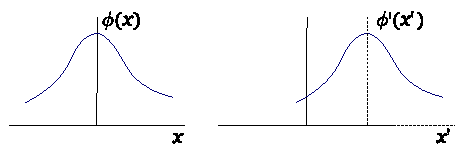
\includegraphics{trasla} %noinstiki
  \caption{Traslaci\'on de funci\'on y coordenadas en una dimensi\'on: $\phi(x)=\phi'(x')$ } %noinstiki
  \label{fig:trasla} %noinstiki
\end{figure} %noinstiki<div id="fig:trasla">Figura trasla:Traslaci\'on de funci\'on y coordenadas $\phi(x)=\phi(x')$ </div>
%noinstiki![trasla](http://gfif.udea.edu.co/figfs/trasla.png)
%noinstiki
Si $a^\mu$ es constante (un an\'alisis m\'as general es hecho en \cite{r})
\begin{equation}
  d^4x'=d^4x
\end{equation}
En este caso, asumiendo que el campo satisface las ecuaciones de
Euler-Lagrange y usando la ec.~\eqref{eq:dmuxmu} y (\ref{eq:eelcallfmu}) tenemos
\begin{align}
  \delta S&=\int_{R}d^4x\,\mathcal{L}(\phi',\partial_\mu\phi',x')-\int_{R}d^4x\,\mathcal{L}(\phi(x),\partial_\mu\phi(x),x)\nonumber\\
  &=\int_{R}d^4x\,\mathcal{L}(\phi+\delta\phi,\partial_\mu\phi+\partial_\mu(\delta\phi),x+\delta a)-\int_{R}d^4x\,\mathcal{L}\nonumber\\
  &\approx\int_{R}d^4x\,
  \left[\mathcal{L}+
    \frac{\partial\mathcal{L}}{\partial\phi}\delta\phi+\frac{\partial\mathcal{L}}{\partial(\partial_\mu\phi)}\partial_\mu(\delta\phi)+
    (\partial_\mu\mathcal{L})\delta a^\mu\right]-\int_{R}d^4x\,\mathcal{L}\nonumber\\
  &=\int_{R}d^4x\,
  \left[
    \frac{\partial\mathcal{L}}{\partial\phi}\delta\phi+\frac{\partial\mathcal{L}}{\partial(\partial_\mu\phi)}\partial_\mu(\delta\phi)+
    (\partial_\mu\mathcal{L})\delta a^\mu\right]\nonumber\\
  &=\int_{R}d^4x\,
  \left\{ 
    \left[\partial_\mu\left(\frac{\partial\mathcal{L}}{\partial(\partial_\mu\phi)}
    \right)\right]\delta\phi+\frac{\partial\mathcal{L}}{\partial(\partial_\mu\phi)}\partial_\mu(\delta\phi)+
    (\partial_\mu\mathcal{L})\delta a^\mu\right\}\nonumber\\
  &=\int_{R}d^4x\left\{ 
    \partial_\mu\left[\frac{\partial\mathcal{L}}{\partial(\partial_\mu\phi)}\delta\phi\right]
  +(\partial_\mu\mathcal{L})\delta a^\mu\right\}\nonumber\\
  &=\int_{R}d^4x\,
    \partial_\mu\left[
      -\frac{\partial\mathcal{L}}{\partial(\partial_\mu\phi)}(\partial_\nu\phi)
      +\delta^\mu_\nu\mathcal{L}
    \right]\delta a^\nu\nonumber\\
    \label{eq:2}
  &=\int_{R}d^4x\,
  \left(
    \partial_\mu T^\mu_\nu
  \right)\delta a^\nu=0.
\end{align}
Y por consiguiente
\begin{equation}
  \label{eq:131}
  \partial_\mu T^\mu_\nu=0,
\end{equation}
donde
\begin{equation}
  \label{eq:tmunu}
    T^\mu_\nu=\frac{\partial\mathcal{L}}{\partial(\partial_\mu\phi)}(\partial_\nu\phi)
      -\delta^\mu_\nu\mathcal{L}
\end{equation}
El tensor $T^\mu_\nu$ proviene de asumir la homogeneidad del espacio y el tiempo y es llamado el tensor de momentum--energ\'\i a. 
La densidad Hamiltonina se obtiene de $T^0_0$
\begin{align}
  \label{eq:3}
\mathcal{H}&=T^0_0=\frac{\partial\mathcal{L}}{\partial\dot{\phi}}\dot{\phi}
      -\mathcal{L}\\
      &=\pi(x)\frac{\partial\phi(x)}{\partial t}-\mathcal{L}.
\end{align}
Comparando con la expresi\'on correspondiente en la formulaci\'on
Lagrangiana de la Mec\'anica Cl\'asica, tenemos que si $\phi(x)$ es la
variable can\'onica, la variable can\'onica conjugada es $\pi(x)$
\begin{equation}
  \label{eq:4}
  \pi(x)=\frac{\partial\mathcal{L}}{\partial(\partial\phi(x)/\partial t)}.
\end{equation}
El teorema de Noether en este caso establece que la invarianza de la Acci\'on bajo traslaciones temporales da lugar a la ecuaci\'on de continuidad (\ref{eq:131}) para $\nu=0$
\begin{align}
\label{eq:122}
  \partial_\mu T^\mu_0=0
\end{align}
cuya carga conservada corresponde a la energ\'\i a
\begin{align}
  H=\int_V d^3x\, T^0_0=\int_V d^3x\,\mathcal{H}.
\end{align}
De igual forma la invarianza bajo traslaciones espaciales de lugar a ecuaciones de continuidad para cada componente $\nu=i$
 ($i=1,2,3$)
 \begin{align}
   \label{eq:235}
   \partial_\mu T^\mu_i=0,
 \end{align}
cuyas densidad de cargas conservadas, $T^0_i$, que en forma vectorial escribiremos como $\mathbf{T}^0$, dan lugar a la conservaci\'on del momentum
\begin{align}
  \mathbf{P}=\int_V d^3x\,\mathbf{T}^0\,.
\end{align}
Generalizando a un campo complejo
\begin{equation}
  \label{eq:138}
     T^\mu_\nu=\frac{\partial\mathcal{L}}{\partial(\partial_\mu\phi)}(\partial_\nu\phi)+(\partial_\nu\phi^*)\frac{\partial\mathcal{L}}{\partial(\partial_\mu\phi^*)}
      -\delta^\mu_\nu\mathcal{L}
\end{equation}

\section{Aplicaci\'on a Mec\'anica Cu\'antica}
\label{sec:aplic-mecan-cuant}

Haciendo $\hbar=1$, el Lagrangiano que da lugar a la ecuaci\'on de Schr\"odinger es
\begin{align}
\label{eq:5}
  \mathcal{L}(\psi,\psi^*,\partial_\mu\psi,\partial_\mu\psi^*)&=\frac{1}{2m}\boldsymbol{\nabla}\psi^*\cdot\boldsymbol{\nabla}\psi-\frac{i}{2}
  \left(
\psi^*\frac{\partial\psi}{\partial t}-\frac{\partial\psi^*}{\partial t}\psi
  \right)+\psi^*V\psi\\
&=\frac{1}{2m}\partial_i\psi^*\partial_i\psi-\frac{i}{2}
  \left(\psi^*\partial_0\psi-\partial_0\psi^*\psi\right)+\psi^*V\psi.\nonumber
\end{align}
Aplicando las ecuaciones de Euler-Lagrange (\ref{eq:132}) para
la funci\'on de onda $\psi^*$ obtenemos la ecuaci\'on de Scr\"odinger con $\hbar=1$:
\begin{equation}
  \label{eq:137}
    0=\partial_\mu\left[\frac{\partial\mathcal{L}}{\partial(\partial_\mu\psi^*)}\right]-\frac{\partial\mathcal{L}}{\partial\psi^*}=
  \partial_0\left[\frac{\partial\mathcal{L}}{\partial(\partial_0\psi^*)}\right]+  
\partial_i\left[\frac{\partial\mathcal{L}}{\partial(\partial_i\psi^*)}\right]-\frac{\partial\mathcal{L}}{\partial\psi^*}.
\end{equation}
Como
\begin{align}
  \label{eq:136}
  &\frac{\partial\mathcal{L}}{\partial(\partial_0\psi)}=-\frac{i}{2}\psi^*&&\frac{\partial\mathcal{L}}{\partial(\partial_0\psi^*)}=\frac{i}{2}\psi\nonumber\\
  &\frac{\partial\mathcal{L}}{\partial(\partial_i\psi)}=\frac{1}{2m}\partial_i\psi^*&&\frac{\partial\mathcal{L}}{\partial(\partial_i\psi^*)}=\frac{1}{2m}\partial_i\psi\\
  &\frac{\partial\mathcal{L}}{\partial\psi}=\frac{i}{2}\partial_0\psi^*+\psi^*V&&\frac{\partial\mathcal{L}}{\partial\psi^*}=-\frac{i}{2}\partial_0\psi+V\psi.\nonumber
\end{align}
Entonces, reemplazando la ec.~(\ref{eq:136}) en la ec.~(\ref{eq:137}), tenemos
\begin{align}
 0=\partial_\mu\left[\frac{\partial\mathcal{L}}{\partial(\partial_\mu\psi^*)}\right]-\frac{\partial\mathcal{L}}{\partial\psi^*}
 &=\partial_0\left(\frac{i}{2}\psi\right)+\partial_i\left(\frac{1}{2m}\partial_i\psi\right)
  -\left(-\frac{i}{2}\partial_0\psi+V\psi\right)\nonumber\\
  &=\frac{i}{2}\partial_0\psi+\frac{1}{2m}\partial_i\partial_i\psi+\frac{i}{2}\partial_0\psi-V\psi.
\end{align}

Que puede escribirse como
\begin{equation}
  \label{eq:133}
  i\frac{\partial}{\partial t}\psi=
  \left(
    -\frac{1}{2m}\nabla^2+V
  \right)\psi.
\end{equation}

El Lagrangiano en ec~(\ref{eq:5}), y por consiguiente la Acci\'on, es invariante bajo una transformaci\'on de fase
\begin{equation}
  \label{eq:6}
  \psi\to\psi'=e^{i\theta}\psi.
\end{equation}
Por consiguiente, de acuerdo al Teorema de Noether, debe existir una cantidad conservada. La corriente conservada se obtine de la ec.~(\ref{eq:jmuphi}). Para los campos $\psi$ y $\psi^*$, tenemos
\begin{align}
  \delta\psi=\psi'-\psi=(e^{i\theta}-1)\psi&\approx i\theta\psi\\
  \delta\psi^*&\approx-i\theta\psi.
\end{align}
Usando adem\'as la ec.~(\ref{eq:136}) en la definici\'on de $J^0$ dada por la ec.~(\ref{eq:jmuphi}), tenemos
\begin{align}
  \label{eq:135}
  J^0&=\left[\frac{\partial\mathcal{L}}{\partial(\partial_0\psi)}\right]\delta\psi
  +\delta\psi^*\left[\frac{\partial\mathcal{L}}{\partial(\partial_0\psi^*)}\right]\nonumber\\
  &=-\frac{i}{2}\psi^*(i\theta\psi)+(-i\theta\psi^*)\frac{i}{2}\psi\nonumber\\
  &=\theta\psi^*\psi,
\end{align}
y
\begin{align}
  \label{eq:134}
  J^i&=\left[\frac{\partial\mathcal{L}}{\partial(\partial_i\psi)}\right]\delta\psi
  +\delta\psi^*\left[\frac{\partial\mathcal{L}}{\partial(\partial_i\psi^*)}\right]\nonumber\\
  &=\frac{1}{2m}\partial_i\psi^*(i\theta\psi)+(-i\theta\psi^*)\frac{1}{2m}\partial_i\psi\nonumber\\
  &=\frac{i\theta}{2m}\left(\partial_i\psi^*\psi-\psi^*\partial_i\psi \right).
\end{align}
Entonces, normalizando apropiadamente la corriente escogiendo $\theta=1$, tenemos
\begin{align}
  \label{eq:7}
  J^0&=\psi^*\psi\\
  \mathbf{J}&=\frac{i}{2m}
  \left(
    \psi\boldsymbol{\nabla}\psi^*-\psi^*\boldsymbol{\nabla}\psi
  \right).
\end{align}
De acuerdo a la ec.~(\ref{eq:7}), la cantidad conservada corresponde a la probabilidad de la funci\'on de onda y normalizando apropiadamente la ec.~(\ref{eq:qcons})
\begin{equation}
  \label{eq:57}
Q_\rho=  \int_V \psi^*\psi \,d^3x=1.
\end{equation}


En cuanto a las simetr\'\i as externas, tenemos de la ec.~(\ref{eq:tmunu}) que
da lugar a las ecuaciones de continuidad (\ref{eq:122})(\ref{eq:235})
\begin{align}
  \partial_\mu T^\mu_0&=0,\nonumber\\
\partial_\mu{T}^\mu_i&=0
\end{align}
Las cargas conservadas se pueden obtener de las densidades de carga
$T^0_0$ y $T^0_i$. 

\subsection{Conservación del moméntum}
Comencemos con las densidades de carga asociadas a
la conservación del moméntum lineal.
Usando  las ecs.~(\ref{eq:136}) en la ec.~(\ref{eq:138})
\begin{align}
  T^0_i=&\frac{\partial\mathcal{L}}{\partial(\partial_0\psi)}(\partial_i\psi)
  +(\partial_i\psi^*)\frac{\partial\mathcal{L}}{\partial(\partial_0\psi^*)}\nonumber\\
  T^0_i=&-\frac{i}{2}\psi^*(\partial_i\psi)+\frac{i}{2}(\partial_i\psi^*)\psi
\end{align}
Entonces, definiendo
\begin{equation}
   \mathbf{T}^0=\frac{i}{2}
  \left(
    \psi\boldsymbol{\nabla}\psi^*-\psi^*\boldsymbol{\nabla}\psi
  \right)
\end{equation}
Procedemos ahora a reemplazar $\psi\boldsymbol{\nabla}\psi^*$ por la
derivada total
\begin{align}
 \mathbf{T}^0&=\frac{i}{2}
  \left[\left( 
    \boldsymbol{\nabla}(\psi^*\psi)-\psi^*\boldsymbol{\nabla}\psi \right)-\psi^*\boldsymbol{\nabla}\psi
  \right]\nonumber\\
&=-i\psi^*\boldsymbol{\nabla}\psi+\frac{i}{2}\boldsymbol{\nabla}(\psi^*\psi)\,.
\end{align}
Integrando en el volumen
\begin{equation}
  \int_V \mathbf{T}^0\, d^3x=-i\int_V \psi^*\boldsymbol{\nabla}\psi\, d^3x+\frac{i}{2}\boldsymbol{\nabla}\int_V\psi^*\psi\,d^3x
\end{equation}
De acuerdo a la ec.~(\ref{eq:57}), la \'ultima integral es una constante y
\begin{align}
  \label{eq:140}
  \int_V \mathbf{T}^0\, d^3x=-i\int_V \psi^*\boldsymbol{\nabla}\psi d^3x\nonumber\\
\langle\widehat{\mathbf{p}}\rangle=\int_V \psi^*\widehat{\mathbf{p}}\psi d^3x
\end{align}
De modo que $\langle\widehat{\mathbf{p}}\rangle$ son las cargas conservadas asociadas al valor esperado el operador de momentum
\begin{equation}
  \widehat{\mathbf{p}}=-i\boldsymbol{\nabla}\,.
\end{equation}
En general, el valor esperado de un operador $ \widehat{\cal O}$, se define en mecánica cuántica como
\begin{align*}
  \langle\widehat{\cal O}\rangle=\int_V d^3x\,\psi^{*}\widehat{\cal O}\psi\,.
\end{align*}

\subsection{Conservación de la energía}
De otro lado
\begin{align}
  T^0_0&=\frac{\partial\mathcal{L}}{\partial(\partial_0\psi)}{\partial_0\psi}+{\partial_0\psi^*}\frac{\partial\mathcal{L}}{\partial(\partial_0\psi^*)}-\mathcal{L}\nonumber\\
  &=-\frac{i}{2}\psi^*\partial_0\psi+\frac{i}{2}\partial_0\psi^*\psi-\frac{1}{2m}\partial_i\psi^*\partial_i\psi+\frac{i}{2}
  \left(\psi^*\partial_0\psi-\partial_0\psi^*\psi\right)-\psi^*V\psi\nonumber\\
  &=-\frac{1}{2m}\partial_i\psi^*\partial_i\psi-\psi^*V\psi
\end{align}
Como las corrientes solo est\'an determinadas hasta un factor de proporcionalidad, definimos
\begin{align}
  \label{eq:139}
   \mathcal{H}&\equiv-T^0_0=\frac{1}{2m}\boldsymbol{\nabla}\psi^*\cdot\boldsymbol{\nabla}\psi+\psi^*V\psi\nonumber\\
   &=\frac{1}{2m}\boldsymbol{\nabla}\cdot(\psi^*\boldsymbol{\nabla}\psi)-\frac{1}{2m}\psi^*\nabla^2\psi+\psi^*V\psi.
\end{align}
Integrando sobre el volumen y usando la ec.~(\ref{eq:140})
\begin{align}
 \int_V\mathcal{H}\,d^3x&=\frac{1}{2m}\int_V\boldsymbol{\nabla}\cdot(\psi^*\boldsymbol{\nabla}\psi)
+\int_V\psi^*\left(-\frac{1}{2m}\nabla^2+V\right)\psi\,d^3x\nonumber\\
&=\frac{1}{2m}\boldsymbol{\nabla}\cdot\int_V(\psi^*\boldsymbol{\nabla}\psi)
+\int_V\psi^*\left(-\frac{1}{2m}\nabla^2+V\right)\psi\,d^3x\nonumber\\
&=\frac{i}{2m}\boldsymbol{\nabla}\cdot\langle\widehat{\mathbf{p}}\rangle
+\int_V\psi^*\left(-\frac{1}{2m}\nabla^2+V\right)\psi\,d^3x\nonumber\\
&=\int_V\psi^*\left(-\frac{1}{2m}\nabla^2+V\right)\psi\,d^3x\,.
\end{align}

Entonces
\begin{align}
\label{eq:141}
H&\equiv \int_V\mathcal{H}\,d^3x=\int_V\psi^*\left(-\frac{1}{2m}\nabla^2+V\right)\psi\,d^3x\nonumber\\
&=\int_{V} d^3x\,\psi^*\widehat{H}\psi=\langle\widehat{H}\rangle.
\end{align}
Que es un resultado bien conocido de la mec\'anica cu\'antica.

Como
\begin{equation}
  \widehat H=\frac{1}{2m}\hat p^2+\widehat V,
\end{equation}
podemos escribir la ec.~(\ref{eq:133}) como
\begin{equation}
  i\frac{\partial}{\partial t}\psi=\widehat H \psi\,.
\end{equation}
Podemos identificar entonces los operadores de energ\'\i a y momentum.
\begin{equation}
  \label{eq:151}
  \widehat H=i\frac{\partial}{\partial t},\qquad \hat{\mathbf{p}}=-i\,\boldsymbol{\nabla}.
\end{equation}

Retornando a la ec.~(\ref{eq:140}), tenemos que para la soluci\'on de part\'\i cula libre de la ecuaci\'on de Schr\"odinger 
\begin{equation}
  \psi=A\,e^{-i\mathbf{k}\cdot\mathbf{x}},
\end{equation}
la condici\'on de normalizaci\'on en ec.~\eqref{eq:57} implica que $|A|^2=1/L^3$, y
\begin{align}
  \int_V \mathbf{T}^0\, d^3x&=\mathbf{k}.
\end{align}

\begin{itemize}
\item[\textbf{Ejercicio:}]  De la ec.~(\ref{eq:141}) obtenega la densidad Hamiltoniana, y usando la ec.~(\ref{eq:3}) encontrar la densidad Lagrangiana~\eqref{eq:5}.
\end{itemize}


\section{Invarianza de fase local del Lagrangiano de  Scrödinger's}

%Trasladar el material de sección 3.4 aquí. 

When we discuss the wave function $\psi(x)$, $x$ represents the point in space at which we want to know the value of the wave function. Since complex numbers are, well, complex, you can't represent them by a position on a simple number line. Instead, the have to be represented by a point in a two--dimensional plot. 

In addition the length of the arrow pointing to the complex number we also need an angle to specify exactly how to draw the arrow pointing to the complex number. The observable is encoded into the length of the arrow representing the value of the complex valued wave function at that point of the space--time. Its angle is unobservable.

The complex number $\psi(x)$ in the Scrödinger equation is just the number whose square is the relative probability of finding the object at that point.

Now, suppose that you arbitrarily decide to make a change of phase of the wave function --to change, at every point in space, the angle $\theta$ of the complex number $\psi$ makes with the real axis. Here is the critical point: Is this change phase is \emph{global}, if the phase that you change the phase angle $\theta$ is the same everywhere in space, the this change of phase will not destroy the delicate and essential balance between the kinetic and potential energy in the Scrödinger equation.

However, in the view implemented by Einstein's relativity, the need to require that quantum--mechanical systems be unaltered only by global changes of phase seemed to be very unnatural. Once you choose the phase of the wave function at one space-time point, the requirement of global phase invariance fixes it at all other space-time points:


  \begin{quote}
\small
    As usually conceived however, this arbitrariness is subject to the following  limitation: once one choose [the phase of the wave function] at one space--time point, one is then not free to make any choices at other space--time points.

It seems that it is not consistent with the localized field concept that underlies the usual physical theories. In the present paper we wish to explore the possibility of requiring all the interactions to be invariant under independent [change of phases] at all space-time points.
  \end{quote}
  \begin{flushright}
    Yang-Mills, \emph{Physical Review}, 1954
  \end{flushright}

This is similar to what happens in electromagnetic theory expressed in terms of scalar and vector potentials. The can be changed by arbitrary functions in a such way that the measured electric and magnetic fields remain invariant. As we will see, this feature is deeply connected with the local conservation of electric charge. 

We start again with the Scrödinger Lagrangian as written in eq.~\eqref{eq:5qft}: but without the interaction term

\begin{align}
  \mathcal{L}(\psi,\psi^*,\partial_\mu\psi,\partial_\mu\psi^*)&=\frac{1}{2m}\boldsymbol{\nabla}\psi^*\cdot\boldsymbol{\nabla}\psi-\frac{i}{2}
  \left(
\psi^*\frac{\partial\psi}{\partial t}-\frac{\partial\psi^*}{\partial t}\psi
  \right)+\cancel{\psi^*V\psi}\\
\mathcal{L}_{\text{free}}&=\frac{1}{2m}\partial_i\psi^*\partial_i\psi-\frac{i}{2}
  \left(\psi^*\partial_0\psi-\partial_0\psi^*\psi\right).\nonumber
\end{align}
This Lagrangian is not invariant under local phase changes of the wave function: 
\begin{align}
  \partial_\mu \psi\to\partial_\mu \psi'=&\partial_\mu \left(e^{i\theta(x)}\psi\right)\nonumber\\
  =&\left(\partial_\mu e^{i\theta(x)}\right)\psi+e^{i\theta(x)}\partial_\mu\psi\nonumber\\
  =&e^{i\theta(x)}\left(i\partial_\mu \theta(x)\right)\psi+e^{i\theta(x)}\partial_\mu\psi\nonumber\\
  =&e^{i\theta(x)}\left[i\partial_\mu \theta(x)+\partial_\mu\right]\psi\,.
\end{align}
In order to have a new Lagrangian invariant under local phase changes, or local gauge transformations, we need to introduce a new term to compensate for the term arising from the derivate of $e^{i\theta(x)}$:
\begin{align}
\label{eq:165qft}
   \mathcal{D}_\mu \psi\to\mathcal{D}_\mu' \psi'=&(\partial_\mu+X'_\mu) \left(e^{i\theta(x)}\psi\right)\nonumber\\
   =&e^{i\theta(x)}\left[i\partial_\mu \theta(x)+\partial_\mu\right]\psi+X'_\mu \left(e^{i\theta(x)}\psi\right)\nonumber\\
   =&e^{i\theta(x)}\left[i\partial_\mu \theta(x)+\partial_\mu+X'_\mu \right]\psi\,.
\end{align}
The transformation condition of the new term $X_\mu$, in order to compensate for the term arising from the derivative of the local phase, $i\partial_\mu\theta(x)$, is just that
\begin{align}
\label{eq:169qft}
X_\mu\to  X'_\mu=X_\mu-i\partial_\mu\theta(x)\,.
\end{align}
Replacing back in Eq.~\eqref{eq:165qft} we have
\begin{align}
    \mathcal{D}_\mu \psi\to\left(\mathcal{D}_\mu \psi\right)'=\mathcal{D}_\mu' \psi'=&(\partial_\mu+X'_\mu) \left(e^{i\theta(x)}\psi\right)\nonumber\\
=&e^{i\theta(x)}\left[i\partial_\mu \theta(x)+\partial_\mu+X_\mu-i\partial_\mu\theta(x) \right]\psi\nonumber\\
=&e^{i\theta(x)}\left[\partial_\mu+X_\mu\right]\psi\nonumber\\
=&e^{i\theta(x)}\left(\mathcal{D}_\mu\psi\right)\,.
\end{align}
Note that $\mathcal{D}_\mu\psi$ transforms like the field $\psi$, and because of this is called the \emph{covariant derivative} of $\psi$.
Similarly
\begin{align}
    (\mathcal{D}_\mu \psi)^*\to{\left(\mathcal{D}_\mu \psi\right)'}^*=&(\partial_\mu+{X'_\mu}^*) \left(\psi^*e^{-i\theta(x)}\right)\nonumber\\
=&\left[-i\partial_\mu \theta(x)+\partial_\mu+X_\mu^*+i\partial_\mu\theta(x) \right]\psi^*e^{-i\theta(x)}\nonumber\\
=&\left[\partial_\mu+X_\mu^*\right]\psi^*e^{-i\theta(x)}\nonumber\\
=&\left(\mathcal{D}_\mu\psi\right)^*e^{-i\theta(x)}\,.
\end{align}

It is convenient to redefine $X_\mu$ in terms of $A_\mu$:
\begin{align}
  A_\mu\equiv\frac{1}{i q}X_\mu\,,
\end{align}
such that the covariant derivative can be conveniently written as
\begin{align}
\label{eq:170qft}
  \mathcal{D}_\mu=\partial_\mu+i q A_\mu\,.
\end{align}
The transformation properties of $A_\mu$ can be obtained from the $X_\mu$ transformation in eq.~\eqref{eq:169qft}: 
\begin{align}
\label{eq:159qft}
 i q A_\mu\to& i q A_\mu'=i q A_\mu-i \partial_\mu\theta(x)\nonumber\\
  A_\mu\to&  A_\mu'= A_\mu-\frac{1}{q} \partial_\mu\theta(x)\,.
\end{align}


We define \emph{local gauge invariance} as an arbitrary way of choosing the complex phase factor of a charged field\footnote{like the electron field as described by the usual Scrödinger equation.} at all space time points.

In this way, we can change the original Lagrangian for a new one which is invariant under local phase transformations:
\begin{align}
   \mathcal{L}(\psi,\psi^*,\partial_\mu\psi,\partial_\mu\psi^*,A_\mu)
=\frac{1}{2m}\left(\mathcal{D}_i\psi\right)^*\mathcal{D}_i\psi-\frac{i}{2}
  \left[\psi^*\mathcal{D}_0\psi-\left(\mathcal{D}_0\psi\right)^*\psi\right].
\end{align}
where
\begin{align}
\label{eq:167qft}
  A_\mu\to A'_\mu=A_\mu-\frac{1}{q}\partial_\mu\theta(x)\,.
\end{align}
This is just the gauge transformation which left the Electromagnetic fields invariant. In fact, the new Lagrangian is now invariant under the local phase transformations
\begin{align}
  \mathcal{L}\to \mathcal{L}'=&
\frac{1}{2m}{\left(\mathcal{D}_i\psi\right)'}^*\left(\mathcal{D}_i\psi\right)'
-\frac{i}{2}\left[{\psi'}^*\left(\mathcal{D}_0\psi\right)'-{\left(\mathcal{D}_0\psi\right)'}^*\psi'\right]\nonumber\\
=&
\frac{1}{2m}{\left(\mathcal{D}_i\psi\right)}^*e^{-i\theta(x)}e^{i\theta(x)}\left(\mathcal{D}_i\psi\right)\nonumber\\
&-\frac{i}{2}\left[{\psi}^*e^{-i\theta(x)}e^{i\theta(x)}\left(\mathcal{D}_0\psi\right)
-{\left(\mathcal{D}_0\psi\right)}^*e^{-i\theta(x)}e^{i\theta(x)}\psi\right].\nonumber\\
=&\mathcal{L}\,.
\end{align}

To preserve invariance one notices that it is necessary to counteract the variation of $\theta$ with $x$, $y$, $z$, and $t$ by introducing the electromagnetic field $A_\mu$. In this way, the electromagnetic interaction is obtained as the result of impose local gauge invariance under $U(1)$ (local phase transformations). To fully implement the gauge principle, i.e, the paradigm to obtain the interactions as the result of the gauge invariance, we need to introduce some concepts of special relativity to be developed below.



\section{Ecuación de Scrödinger en presencia de un campo electromagnético}

The expansion of the Lagrangian in terms of the field $\psi$, $\psi^*$, and $A_\mu$ is 
\begin{align}
\label{eq:178qft}
   \mathcal{L}
=&\frac{1}{2m}\sum_i\left(\partial_i\psi+i q A_i\psi\right)^*\left(\partial_i\psi+i q A_i\psi\right)-\frac{i}{2}
  \left[\psi^*\left(\partial_0\psi+i q A_0\psi\right)-\left(\partial_0\psi+i q A_0\psi\right)^*\psi\right] 
\nonumber\\
=&\frac{1}{2m}\sum_i\left(\partial_i\psi^*-i q A_i\psi^*\right)\left(\partial_i\psi+i q A_i\psi\right)-\frac{i}{2}
  \left[\psi^*\left(\partial_0\psi+i q A_0\psi\right)-\left(\partial_0\psi^*-i q A_0\psi^*\right)\psi\right]
\nonumber\\
 =&\frac{1}{2m}\sum_i\left(\partial_i\psi^*\partial_i\psi-i q \psi^*A_i\partial_i\psi+i q \partial_i\psi^*A_i\psi+q^2A_i A_i \psi^*\psi\right)\nonumber\\
 &-\frac{i}{2}
  \left[\psi^*\partial_0\psi+i q \psi^*A_0\psi-(\partial_0\psi^*)\psi+i q A_0\psi^*\psi\right]\nonumber\\
 =&\frac{1}{2m}\sum_i\left(\partial_i\psi^*\partial_i\psi-i q \psi^*A_i\partial_i\psi+i q \partial_i\psi^*A_i\psi+q^2A_i A_i \psi^*\psi\right)\nonumber\\
 &-\frac{i}{2}
  \left[\psi^*\partial_0\psi-(\partial_0\psi^*)\psi+2 i q \psi^*A_0\psi\right]\,.
 \end{align}

Then we have
\begin{align}
  \mathcal{L}=&\frac{1}{2m}\sum_i\partial_i\psi^*\partial_i\psi
-\frac{i}{2}
  \left[\psi^*\partial_0\psi-(\partial_0\psi^*)\psi\right] \nonumber\\
&+\frac{1}{2m}\sum_i\left[ -i q \psi^*A_i\partial_i\psi+i q \left(\partial_i\psi^*\right) A^i\psi+q^2A_i A_i \psi^*\psi\right]\nonumber\\
 &+ q \psi^*A_0\psi\,.
 \end{align}

From this we can obtain the Euler-Lagrange equation for each field.

In the following developments we will heavily the following notation for vectors, which is going to be explained in next section
\begin{align*}
  \mathbf{A}=\left( A^1,A^2,A^3\right)=-\left( A_1,A_2,A_3\right)\,.
\end{align*}

\subsection{Euler-Lagrange equation for $\psi^*$}
In particular for $\psi^*$ we have
\begin{align}
  \partial_\mu\left[\frac{\partial\mathcal{L}}{\partial(\partial_\mu\psi^*)}\right]-\frac{\partial\mathcal{L}}{\partial\psi^*}=&0\nonumber\\
  \partial_0\left[\frac{\partial\mathcal{L}}{\partial(\partial_0\psi^*)}\right]+\partial_i\left[\frac{\partial\mathcal{L}}{\partial(\partial_i\psi^*)}\right]-\frac{\partial\mathcal{L}}{\partial\psi^*}=&0\nonumber\\
  \frac{i}{2}\partial_0\psi-\frac{1}{2m}\partial_i\left[\partial^i\psi+i q A^i\psi\right]
-\left[-\frac{1}{2m}\left(-i q A_i\partial^i\psi+q^2A_iA^i\psi\right)
-\frac{i}{2}\left(\partial_0\psi+2 i q A_0\psi\right)\right]=&0\nonumber\\
  i\partial_0\psi-q A_0\psi-\frac{1}{2m}\left[\partial_i\left(\partial^i\psi+i q A^i\psi\right)
+i q A_i\left(\partial^i\psi+i q A^i\psi\right)\right]
=&0\nonumber\\
  i(\partial_0+i q A_0)\psi-\frac{1}{2m}(\partial_i+i q A_i)(\partial^i\psi+i q A^i\psi)
=&0\nonumber\\
   i\mathcal{D}_0\psi
  +\frac{1}{2m}\sum_i\mathcal{D}_i\mathcal{D}_i\psi=&0\,,
\end{align}

If we define
\begin{align}
  \boldsymbol{\mathcal{D}}\equiv\boldsymbol{\nabla}-i q \mathbf{A}\,.
\end{align}
we have in components:
\begin{align}
    \boldsymbol{\mathcal{D}}_i=\partial_i-i q A^i\nonumber\\
    \boldsymbol{\mathcal{D}}_i=\partial_i+i q A_i\,.
\end{align}

Then we have the new wave equation:
\begin{align}
  i\mathcal{D}_0\psi=&-\frac{1}{2m}\boldsymbol{\mathcal{D}}\cdot\boldsymbol{\mathcal{D}}\psi\nonumber\\
i\mathcal{D}_0\psi=&-\frac{1}{2m}\boldsymbol{\mathcal{D}}^2\psi\,,
\end{align}

que corresponde a la ecuación de Scrödinger con la derivada normal reemplazada por la derivada covariante.



Expandiendo esta ecuación tenemos 
\begin{align}
\label{eq:175qft}
   i\left(\frac{\partial}{\partial t}+iqA_0\right)\psi
&=-\frac{1}{2m}\sum_i(\partial_i+i q A_i)^2\psi\nonumber\\
   \left(i\frac{\partial}{\partial t}-qA_0\right)\psi
 &=-\frac{1}{2m}\sum_i(\partial_i-i q A^i)^2\psi\nonumber\\
   \left(i\frac{\partial}{\partial t}-q\phi\right)\psi
&=-\frac{1}{2m}(\boldsymbol{\nabla}-i q \mathbf{A})^2\psi\nonumber\\
   \left(\widehat{H}-q\phi\right)\psi
&=-\frac{-i^2}{2m}(\boldsymbol{\nabla}-i q \mathbf{A})^2\psi\nonumber\\
&=\frac{1}{2m}(i\boldsymbol{\nabla}+ q \mathbf{A})^2\psi\nonumber\\
&=\frac{1}{2m}(-i\boldsymbol{\nabla}- q \mathbf{A})^2\psi\nonumber\\
&=\frac{1}{2m}(\widehat{\mathbf{p}}- q \mathbf{A})^2\psi\,.
\end{align}
In this way, the Scrödinger equation in presence of the electromagnetic field, can be obtained from the original Scrödinger equation but with the \emph{minimum substitution}:
\begin{align}
  \widehat{H}\to& \widehat{H}-q\phi & \widehat{\mathbf{p}}\to&\widehat{\mathbf{p}}-q\mathbf{A}\,.
\end{align}



De la ecuación (\ref{eq:175qft}) podemos obtener la ecuación de Schödinger en presencia de un campo electromagnético
\begin{align}
\label{eq:176qft}
 i\frac{\partial}{\partial t}\psi&=\left[\frac{1}{2m}(-i\mathbf{\nabla}-q\mathbf{A})^2+qA_0\right]\psi\,.
\end{align}
 Para que la mecánica cuántica sea consistente con las ecuaciones de Maxwell es necesario que las transformaciones gauge (\ref{eq:159qft}) de los potenciales de Maxwell estén acompañados por una transformación de la función de onda, $\psi\to\psi'$, donde $\psi'$ satisface la ecuación
\begin{align}
  \label{eq:160qft}
   i{\mathcal{D}'}^0\psi'&=-\frac{1}{2m}{\boldsymbol{\mathcal{D}}'}^2\psi'\nonumber\\
 i\frac{\partial}{\partial t}\psi'&=\left[\frac{1}{2m}(-i\mathbf{\nabla}-q\mathbf{A}')^2+q{A'}_0\right]\psi'\,.
\end{align}
Como la forma de la ecuación (\ref{eq:160qft}) es exactamente la misma que la forma de~\eqref{eq:176qft} entonces ambas describen la misma física. Se dice que  la ec.~\eqref{eq:176qft} es covariante gauge, lo que significa que mantiene la misma forma bajo una transformación gauge. 

\begin{itemize}
\item \textbf{Ejemplo:}\\ 
Demuestre que la ec.~\eqref{eq:160qft} es covariante:



Como 
\begin{align}
  \psi\to \psi'=e^{i\theta(x)}\psi
\end{align}
Entonces
\begin{align}
  \boldsymbol{\mathcal{D}}'\psi'&=\left[(\boldsymbol{\nabla}-iq\mathbf{A})-i\boldsymbol{\nabla}\theta\right]e^{i\theta(x)}\psi\nonumber\\
  &=i(\boldsymbol{\nabla}\theta)e^{i\theta(x)}\psi+e^{i\theta(x)}\boldsymbol{\nabla}\psi-iq\mathbf{A}e^{i\theta(x)}\psi-i(\boldsymbol{\nabla}\theta) e^{i\theta(x)}\psi\nonumber\\
  &=e^{i\theta(x)}(\boldsymbol{\nabla}-iq\mathbf{A})\psi\nonumber\\
  &=e^{i\theta(x)}(\boldsymbol{\mathcal{D}}\psi)
\end{align}
y
\begin{align}
  {\boldsymbol{\mathcal{D}}'}^2\psi'&=\boldsymbol{\mathcal{D}}'(\boldsymbol{\mathcal{D}}'\psi')\nonumber\\
  &=\left[(\boldsymbol{\nabla}-iq\mathbf{A})-i\boldsymbol{\nabla}\theta\right]e^{i\theta(x)}(\boldsymbol{\mathcal{D}}\psi)\nonumber\\
  &=i(\boldsymbol{\nabla}\theta)e^{i\theta(x)}(\boldsymbol{\mathcal{D}}\psi)+e^{i\theta(x)}\boldsymbol{\nabla}(\boldsymbol{\mathcal{D}}\psi)
  -iq\mathbf{A}e^{i\theta(x)}(\boldsymbol{\mathcal{D}}\psi)-i\boldsymbol{\nabla}\theta e^{i\theta(x)}(\boldsymbol{\mathcal{D}}\psi)\nonumber\\
  &=e^{i\theta(x)}(\boldsymbol{\nabla}-iq\mathbf{A})(\boldsymbol{\mathcal{D}}\psi)\nonumber\\
  &=e^{i\theta(x)}(\boldsymbol{\mathcal{D}}^2\psi)
\end{align}

De la misma manera
\begin{equation}
  {\mathcal{D}'}^0\psi'=e^{i\theta(x)}(\mathcal{D}^0\psi)
\end{equation}
De modo que
\begin{equation}
  \mathcal{D}^\mu\psi\to {\mathcal{D}'}^\mu\psi'=e^{i\theta(x)}(\mathcal{D}^\mu\psi)
\end{equation}
y la derivada covariante del campo transforma como el campo. Tenemos entonces que 
\begin{align}
  \label{eq:225qft}
     i{\mathcal{D}'}^0\psi'&=-\frac{1}{2m}{\boldsymbol{\mathcal{D}}'}^2\psi'\nonumber\\
     ie^{i\theta(x)}{\mathcal{D}}^0\psi&=-\frac{1}{2m}e^{i\theta(x)}{\boldsymbol{\mathcal{D}}}^2\psi\nonumber\\
     i{\mathcal{D}}^0\psi&=-\frac{1}{2m}{\boldsymbol{\mathcal{D}}}^2\psi
\end{align}
\end{itemize}

En resumen, para 
\begin{equation}
  \mathcal{D}^\mu=\partial^\mu+iqA^\mu
\end{equation}
y reemplazando $\theta\to q\theta$ tenemos
\begin{align}
   A^\mu&\to{A^\mu}'=A^\mu-\partial^\mu\theta(x)\nonumber\\
   \psi&\to \psi'=e^{iq\theta(x)}\psi\nonumber\\
  \mathcal{D}^\mu\psi&\to {\mathcal{D}'}^\mu\psi'=e^{iq\theta(x)}(\mathcal{D}^\mu\psi)\,.
\end{align}
En esta convención $q$ corresponde al \emph{generador} de la transformación y $\theta$ al parámetro de la transformación.
%\left(\right)


\subsection{Conserved currents}
The 4-current can be obtained directly from the Noether's Theorem:

\begin{align}
  J^\mu=&\frac{\partial\mathcal{L}}{\partial_\mu\psi}\delta\psi+\delta\psi^*\frac{\partial\mathcal{L}}{\partial_\mu\psi^*}\nonumber\\
=&\begin{cases}
  \frac{\partial\mathcal{L}}{\partial_0\psi}\delta\psi+\delta\psi^*\frac{\partial\mathcal{L}}{\partial_0\psi^*}&\mu=0\\
  \frac{\partial\mathcal{L}}{\partial_i\psi}\delta\psi+\delta\psi^*\frac{\partial\mathcal{L}}{\partial_i\psi^*}&\mu=i
\end{cases}.
\end{align}

\begin{align}
  J^0=&-\frac{i}{2}\psi^*(iq\theta)\psi-iq\theta\psi^*\frac{i}{2}\psi\nonumber\\
  =&q\theta\psi^*\psi\,,
\end{align}
\begin{align}
  J^i=&\frac{1}{2m}\left[\left(\partial_i-iqA_i\right)\psi^*iq\theta\psi-iq\theta\psi^*\left(\partial_i+iqA_i\right)\psi\right]\nonumber\\
  J^i=&\frac{iq\theta}{2m}\left[\left(\mathcal{D}_i\psi\right)^*\psi-\psi^*\left(\mathcal{D}_i\psi\right)\right]\,.
  \end{align}

When $\theta$ is fixed to 1 as in ec.~\eqref{eq:135qft} to define the probability, we get eq.~\eqref{eq:85qft}.

It is worth to notice that for $T^0_0$, and $T^0_i$ we should obtain
\begin{align}
  \widehat{H}=& i\frac{\partial}{\partial t}-q\phi & \widehat{\mathbf{p}}=&-i\boldsymbol{\nabla}-q\mathbf{A}\,.
\end{align}

The approach to change the Action for a new one invariant under local phase  transformations, is that the electron cannot be longer considered as an isolated \emph{naked} particle. The electron must be always surrounded by some cloud of virtual particles associated with the electromagnetic field in order to guarantee the conservation of the energy and momentum of the system. In general the wave function of the electron can be represented as the exponential of $iEt$ and $i \mathbf{p}\cdot \mathbf{x}$, so that a local phase transformation will change the energy $E$ and the momentum $\mathbf{p}$ of the electron. This changes must be compensated with the corresponding changes in $A_{\mu}$.

Moreover, to be consistent, we could start with the free Lagrangian before the change of the normal derivative by the covariant derivative. The interactions are not longer imposed by hand but a consequence of the improved Action. 


Si modificamos el Lagrangiano en ec.~\eqref{eq:call2}, para incluir un
t\'ermino adicional ($v=c=1$)
\begin{equation}
  \label{eq:14}
  \mathcal{L}(\partial\phi/\partial t,\partial\phi/\partial z)=\frac{1}{2}
\left[
  \left(\frac{\partial\phi}{\partial t}\right)^2-\left(\frac{\partial\phi}{\partial z}\right)^2-m^2\phi^2
\right].
\end{equation}
entonces, la ec.~\eqref{eq:12} es soluci\'on a la ecuaci\'on resultante de
aplicar las ecuaciones de Euler-Lagrange:
\begin{align}
\label{eq:150}
      \frac{\partial^2\phi}{\partial t^2}-\frac{\partial^2\phi}{\partial z^2}+m^2\phi=&0\nonumber\\
      \left(\frac{\partial^2}{\partial t^2}-\frac{\partial^2}{\partial z^2}+m^2
      \right)\phi=&0,
\end{align}
si
\begin{equation}
  \omega^2=k^2+m^2.
\end{equation}
De este modo $m$ puede interpretarse como la masa de la part\'\i cula. 

Generalizando a 3 dimensiones tenemos el Lagrangiano de Klein-Gordon
\begin{align}
  \label{eq:15}
  \mathcal{L}=&\frac{1}{2}
  \left(
\frac{\partial\phi}{\partial t}
  \right)^2-\tfrac{1}{2}\boldsymbol{\nabla}\phi\cdot\boldsymbol{\nabla}\phi-\tfrac{1}{2}m^2\phi^2,
\end{align}
que dan lugar a la ecuaci\'on de Klein-Gordon

\begin{equation}
\label{eq:152}
  \left(
\frac{\partial^2}{\partial t^2}-\nabla^2+m^2
  \right)\phi=0.
\end{equation}

\section{Problemas}
\label{sec:problemas-2}
\renewcommand{\labelenumi}{\thechapter.\theenumi} %noinstiki
\begin{enumerate}
\item Obtenga el Hamiltoniano a partir de Lagrangiano en\eqref{eq:238} y encuentre la expresi\'on para la densidad Lagrangiana en t\'erminos de $\phi$.
\label{item:pch1.0} %noinstiki
\item Demuestre las ecuaciones (\ref{eq:237})(\ref{eq:236}).
\label{item:pch1.1} %noinstiki

\item \textquestiondown Que cambios se requieren al Lagrangiano de la ecuaci\'on de Dirac para que la Acci\'on sea invariante bajo transformaciones Gauge Locales?. Ver secci\'on \ref{sec:aplic-la-mecan}.



\label{item:pch1.3} %noinstiki

\item A partir del Lagrangiano de la Mec\'anica Cu\'antica invariante bajo transformaciones de fase local encuentre la ecuaci\'on de Schr\"odinger en presencia del campo electromagn\'etico. Ver secci\'on \ref{sec:aplic-la-mecan}.
 



\item Calcule $T^i_0$ para el Lagrangiano de Schr\"odinger
  \begin{align}
    T^i_0=&\frac{\partial\mathcal{L}}{\partial(\partial_i \psi)}\partial_0\psi+\partial_0\psi^*\frac{\partial\mathcal{L}}{\partial(\partial_i \psi^*)}\nonumber\\
    =&\frac{1}{2m}\left(\partial_i\psi^*\partial_0\psi+\partial_0\psi^*\partial_i\psi \right)
  \end{align}
De modo que $T^0_i\neq T^i_0$.

\end{enumerate}


\renewcommand{\labelenumi}{\theenumi} %noinstiki
% \left(\right)
%%% Local Variables: 
%%% mode: latex
%%% TeX-master: "fullnotes"
%%% ispell-local-dictionary: "castellano8"
%%% End: 
